\documentclass[11pt]{beamer}
\usetheme{Boadilla}
\usepackage[utf8]{inputenc}
\usepackage{amsmath}
\usepackage{amsfonts}
\usepackage{amssymb}
\usepackage{graphicx}
\usepackage{tabularx}
\usepackage{tikz}
\usetikzlibrary{arrows,shapes.geometric,positioning}
\usepackage{pifont}% http://ctan.org/pkg/pifont
\newcommand{\xmark}{\ding{55}}%
% Define block styles
\tikzstyle{block} = [rectangle, draw, fill=blue!20, 
    text width=9.5em, text centered, rounded corners, minimum height=4em]
\tikzstyle{line} = [draw, -latex]

\graphicspath{{fig/}}

\author[Weiyao Ke]{Weiyao Ke, J Scott Moreland, Jonah E Bernhard, and Steffen A Bass}
\title[3D Initial Condition]{Constraining 3D Hydrodynamic Initial Condition for Relativistic Heavy-ion Collisions from Multiplicity Observables of pA and AA @LHC }
%\setbeamercovered{transparent}
%\setbeamertemplate{navigation symbols}{}
%\logo{qcdlogo.pdf}
\institute{Duke University}
\date{}
%\subject{}
\begin{document}

\begin{frame}
\titlepage
\end{frame}

\section{Initial condition for 3+1D simulation}
\begin{frame}{Initial condition for 3+1D simulation}
\begin{itemize}
\item Relativistic viscous hydrodynamics is one of the key tools to study heavy ion collisions.
\item Hydrodynamics initial condition (complicated): energy/entropy density, fluid velocity, stress tensor...
\item Initial condition uncertainties propagate to the extraction of QGP properties.
\item Continuous progress in first principal calculation of initial condition, but very hard!
\end{itemize}
\begin{center}
\color{red} How does experimental data constrain the 3D initial condition (entropy density).
\end{center}
\end{frame}

\begin{frame}{Longitudinal fluctuations and asymmetries}
\begin{itemize}
\item For midrapidity observables, one usually neglects evolution in the beam direction.
\item For rapidity dependent observables, includes longitudinal fluctuations.
\begin{center}
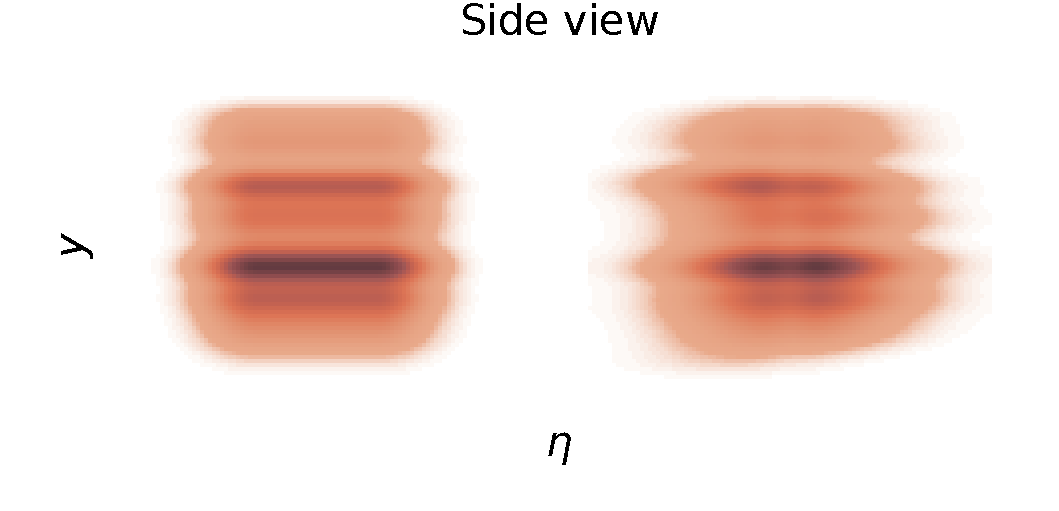
\includegraphics[width=0.6\textwidth]{nuclei_demo.pdf}
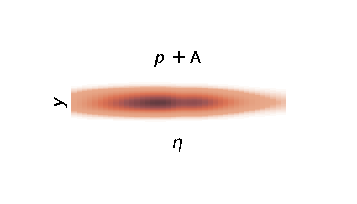
\includegraphics[width=0.3\textwidth]{pPb.pdf} 
\end{center}
\item For small collision system: even stronger asymmetry.
\end{itemize}
\end{frame}

\section{Parametric longitudinal information}
\begin{frame}{At midrapidity: phenomenological model TRENTo }
A brief overview of TRENTo.
\begin{itemize}
\item Nucleons are sampled from Woods-Saxon distribution for nuclei $A, B$.
\item Participants: nucleons participant at least one binary collisions.
\item Nuclear thickness function, $T_{A, B} = \sum_{\textrm{parts A,B}} \Gamma_i \exp\left(-\frac{(r-r_i)^2}{2w^2}\right)$.
\item TRENTo: A family of mappings from nuclear thickness functions $T_A(x_\perp), T_B(x_\perp)$ to midrapidity entropy production $s_0(T_A, T_B)$.
\begin{eqnarray}
\nonumber
s_0(T_A, T_B) \propto \left(\frac{T_A^p + T_B^p}{2}\right)^{1/p}
\end{eqnarray}
$p$ is a tunable continuous parameter that mimics and interpolates between different initial condition models.
\end{itemize}
\end{frame}

\begin{frame}{Extending TRENTo to finite rapidity}
\begin{itemize}
\item The formula,
\begin{eqnarray}\nonumber 
\frac{dS}{dx_\perp^2d y} \propto {\color{red} s_0(\vec{x}_\perp)} {\color{blue}f(y, x_\perp)},
\end{eqnarray} 
\item $s_0$ original TRENTo prediction.
\item {\color{blue} $f(y, x_\perp)$}: rapidity profile with three degrees of freedom,\\
mean ($\mu$), std ($\sigma$), skewness ($\gamma$).
\begin{eqnarray}\nonumber 
f(y) \propto \mathcal{F}^{-1}\exp\left\{ik\mu(x_\perp) -\frac{1}{2}[\sigma(x_\perp) k]^2 - \frac{i}{6}\gamma(x_\perp)[\sigma(x_\perp) k]^3 + ...\right\}
\end{eqnarray}
\item Mean, std, skewness parametrized in nuclear thickness functions.
\end{itemize}
\begin{center}
\begin{tabularx}{0.95\textwidth}{p{2.5cm}p{1.cm}p{8cm}}
\hline
mean & std & absolute or relative-skewness \\
\hline
\noalign{\smallskip}
$\frac{\mu_0}{2} \log\frac{T_A(x_\perp)}{T_B(x_\perp)}$ & $\sigma_0$ & $\gamma_0(T_A(x_\perp)-T_B(x_\perp))$ or $\gamma_0\frac{T_A(x_\perp)-T_B(x_\perp)}{T_A(x_\perp)+T_B(x_\perp)}$ \\
\noalign{\smallskip}
\hline
\end{tabularx}
\end{center}
\end{frame}

\section{Model to data comparison}
\begin{frame}{Model-to-data comparison}
Model: TRENTo-3D, 3+1D Ideal Hydro, Ultra relativistic Quantum Molecular Dynamics (UrQMD)
\begin{itemize}
\item Summary of parameters:\\
"Transverse": normalizations, nucleon width, fluctuation, $p$.\\
"Longitudinal": $\mu_0,\sigma_0, \gamma_0$, Jacobian
\end{itemize}
Data: 
\begin{itemize}
\item Charged particle $\eta$-distribution (ALICE Pb+Pb 2.76TeV, ATLAS $p$+Pb 5.02 TeV), sensitive to centrality/$\eta$ dependent entropy production.
\item Two-particle $\eta$-correlation (ATLAS Pb+Pb 2.76 TeV), 
sensitive to amount of longitudinal fluctuation.
\end{itemize}
*Assume viscous effects on the total multiplicity are mild. Ideal hydro as a crude approximation.
\end{frame}

\begin{frame}{Bayesian model-to-data comparison}
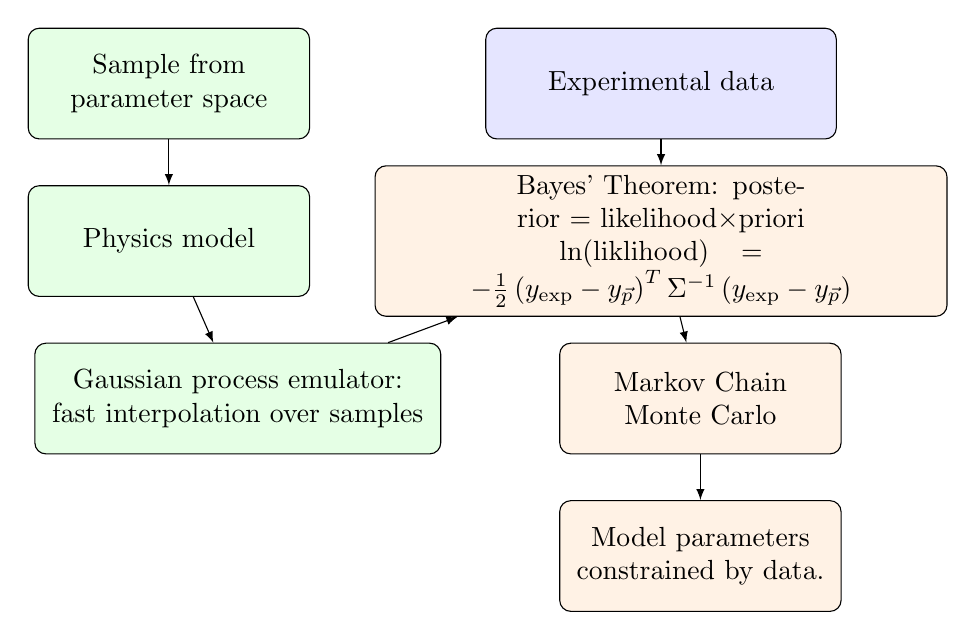
\begin{tikzpicture}[align=center,node distance=4cm]
    % Place nodes
    \node [block, fill=green!10] (param) {Sample from\\ parameter space};
    \node [block, fill=green!10, below of=param, yshift=2cm] (model) {Physics model};
    \node [block, text width=12em, fill=blue!10, right of=param, xshift=2.25cm] (exp) {Experimental data};
    \node [block, text width=14em, fill=green!10, below of=model, xshift=0.875cm, yshift=2cm] (GP) {Gaussian process emulator: fast interpolation over samples};
    \node [block, text width=20em, fill=orange!10, right of=model, xshift=2.25cm] (Bayes) {
    Bayes' Theorem: posterior = likelihood$\times$priori\\ 
    $\ln(\textrm{liklihood}) =  -\frac{1}{2} \left(y_{\textrm{exp}} - y_{\vec{p}} \right)^T \Sigma^{-1} \left(y_{\textrm{exp}} - y_{\vec{p}} \right)$
    };
	\node [block, fill=orange!10, below of=Bayes, xshift=0.5cm, yshift=2cm] (MCMC) {Markov Chain Monte Carlo};
	\node [block, fill=orange!10, below of=MCMC, yshift=2cm] (posterior) {Model parameters constrained by data.};
    % Draw edges
    \path [line] (param)-- (model);
    \path [line] (model) -- (GP);
    \path [line] (GP) -- (Bayes);
    \path [line] (exp) -- (Bayes);
   	\path [line] (Bayes) -- (MCMC);
   	\path [line] (MCMC) -- (posterior);

\end{tikzpicture}
\end{frame}

\section{Constraint initial condition and predictions}
\begin{frame}{After fitting to data: posterior observables}
\begin{itemize}
\item Nicely fit the centrality $\&$ pseudorapidity dependence of $dN_{ch}/d\eta$.
\item It fails $\left\langle a_1^2\right\rangle^{1/2}$ for large centrality.
\end{itemize}
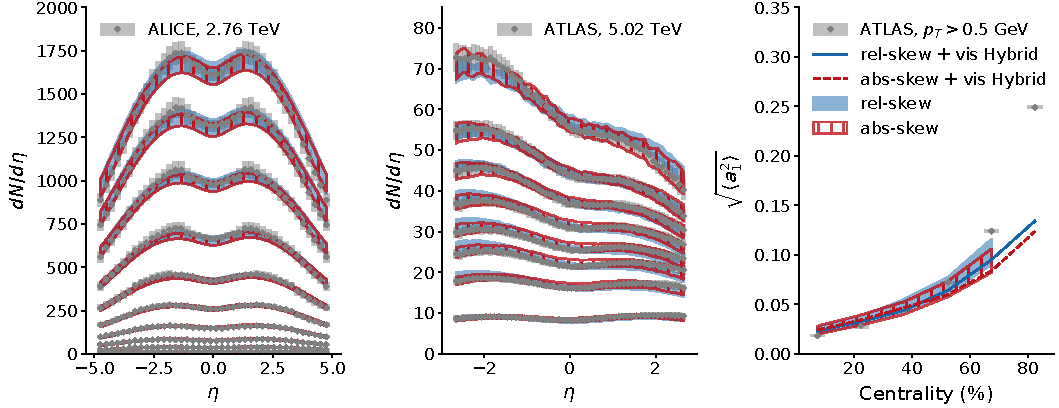
\includegraphics[width=\textwidth]{post_obs.pdf}
\end{frame}

\begin{frame}{Posterior $dS/d\eta$ for various value of $T_A$ and $T_B$}
\begin{itemize}
\item 3D entropy production is reverse engineered from multiplicity data.
\item Figure shows $ds/d\eta(\eta)$ varying $T_A$, $T_B$
\end{itemize}
\begin{center}
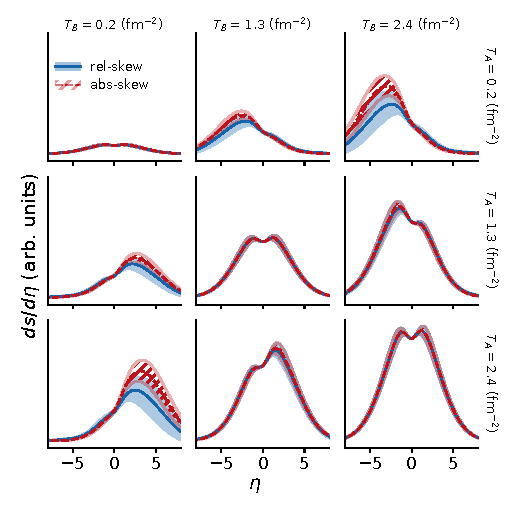
\includegraphics[width=0.6\textwidth]{post_dsdy.pdf}
\end{center}
\end{frame}

\begin{frame}{Calculation of azimuthal correlation observables}
\begin{itemize}
\item We used selected parameters from posterior and viscous hydro + UrQMD to calculate $v_n\{2\}$, and $v_2\{4\}$ and event-plane decorrelations.
\end{itemize}
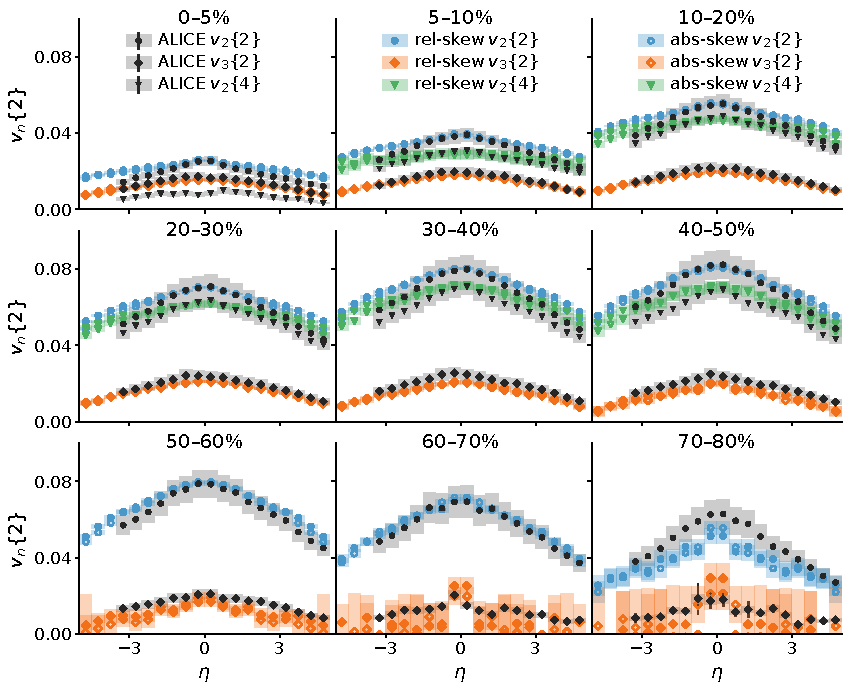
\includegraphics[width=0.59\textwidth]{vn_eta.pdf}\hfill
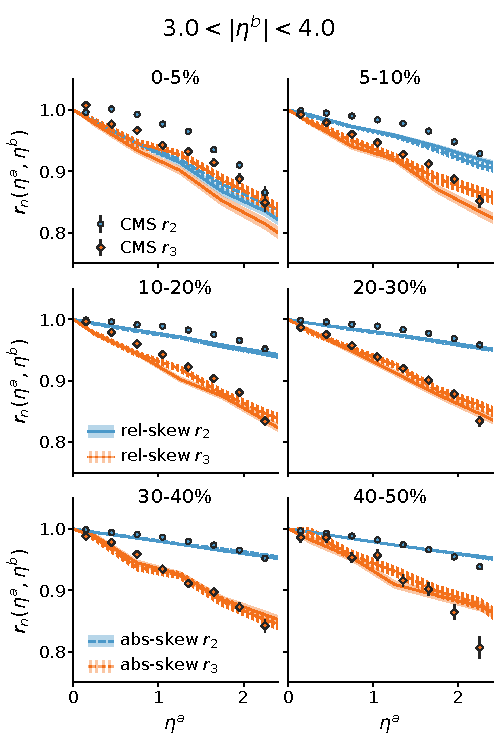
\includegraphics[width=0.325\textwidth]{evt_pln_decorr_near.pdf}
\end{frame}

\begin{frame}{Summary}
\begin{itemize}
\item TRENTo initial condition is extended to include rapidity dependence.
\item A 3D initial condition reverse engineered from data.
\item Could benefit small system simulations.
\end{itemize}
\end{frame}

\begin{frame}{Back up: full nine-parameter posterior}
\begin{center}
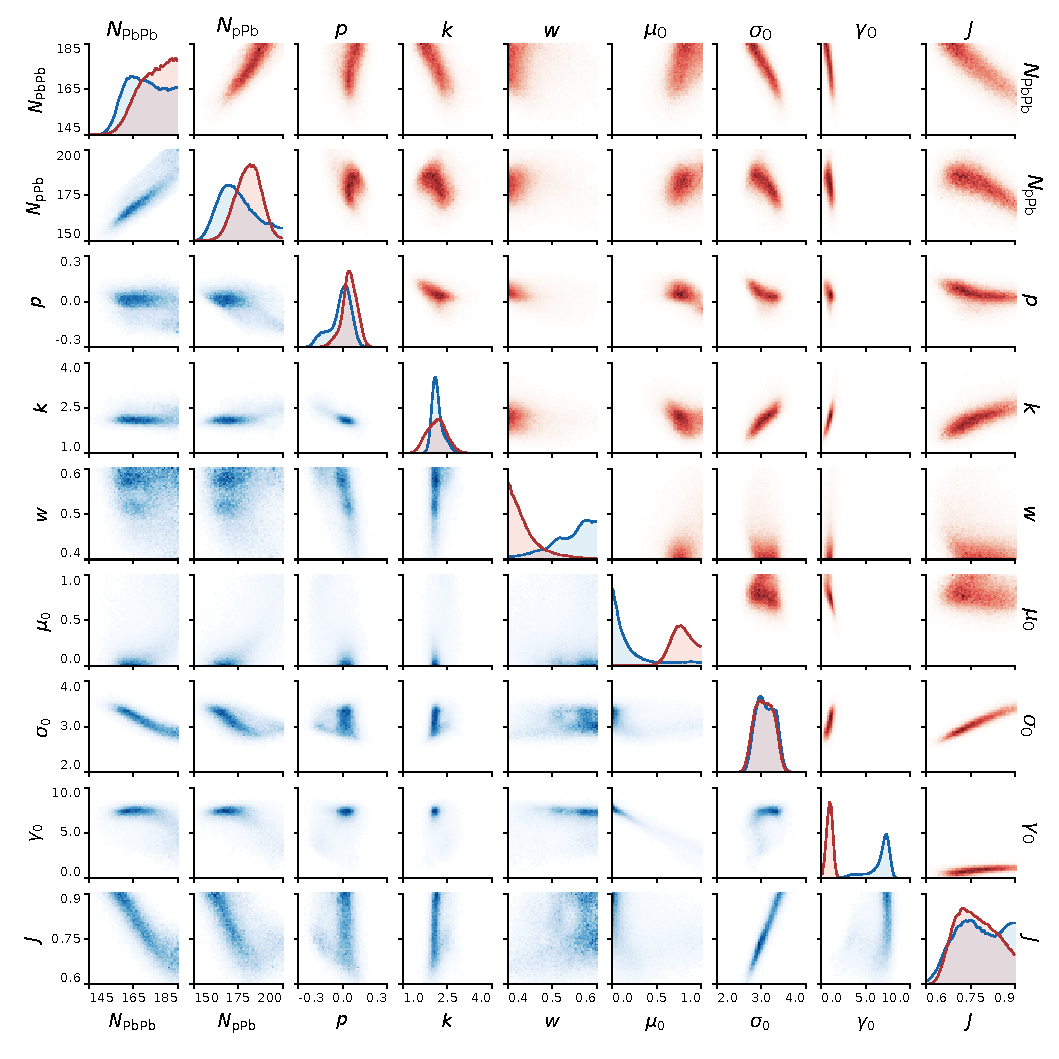
\includegraphics[width=0.7\textwidth]{posterior.pdf}
\end{center}
\end{frame}

\begin{frame}{Back up: Flow at midrapidity}
\begin{center}
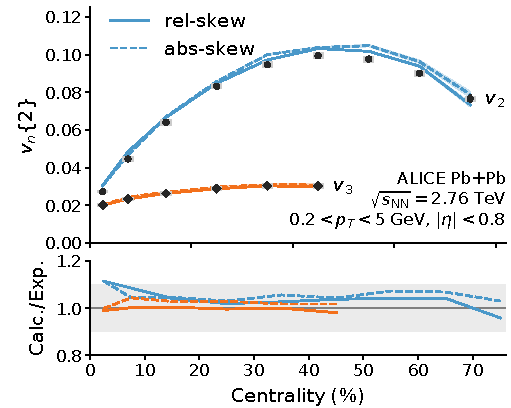
\includegraphics[width=0.8\textwidth]{vn_cen.pdf}
\end{center}
\end{frame}

\begin{frame}{Back up: calculation of symmetric cumulants}
\begin{center}
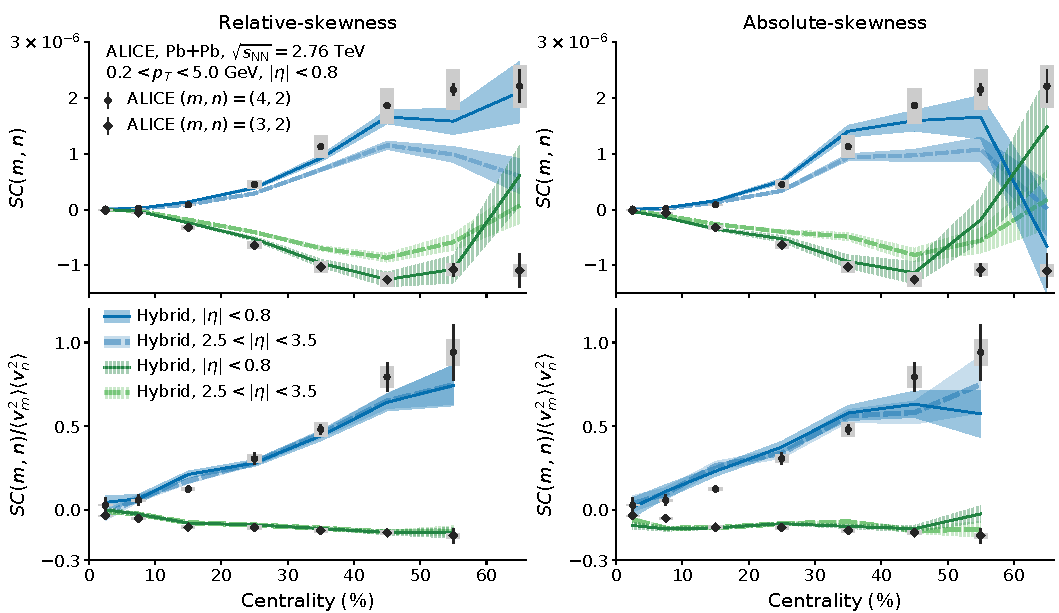
\includegraphics[width=\textwidth]{smn.pdf}
\end{center}
\end{frame}
\end{document}
